\documentclass{article}[11pt]
\usepackage{xparse}
\usepackage{fancyhdr}
\usepackage{pgf,tikz}
\usepackage[utf8]{inputenc}
\usepackage[T1]{fontenc}
\usepackage{listings}
\usepackage{xcolor}
\usepackage{graphicx}
\usepackage{amsmath}
\usepackage[a4paper,left=2cm,right=2cm,top=2.5cm,bottom=2cm]{geometry}
\usepackage{amsmath}
\usepackage{amssymb}
\usepackage{array}
\usepackage{pifont}
\usepackage{makecell}
\usepackage{xcolor}
\usepackage[]{algorithm2e}

% NEW COMMANDS & DEFINE
\definecolor{pythonColor}{HTML}{B634F6}
\definecolor{codegreen}{rgb}{0,0.6,0}
\definecolor{codegray}{rgb}{0.5,0.5,0.5}
\definecolor{codered}{rgb}{1.0,0.2,0.2}
\definecolor{codeyellow}{rgb}{1.0,1.0,0.2}
\definecolor{codepurple}{rgb}{0.58,0,0.82}
\definecolor{backcolour}{rgb}{1.0,1.0,1.0}
\lstdefinestyle{mystyle}{
    backgroundcolor=\color{backcolour},
    commentstyle=\color{codepurple},
    keywordstyle=\color{magenta},
    numberstyle=\tiny\color{codegray},
    stringstyle=\color{codepurple},
    basicstyle=\ttfamily\footnotesize,
    breakatwhitespace=true,
    breaklines=true,
    % captionpos=b,
    keepspaces=true,
    numbers=left,
    numbersep=10pt,
    showspaces=false,
    showstringspaces=false,
    showtabs=false,
    tabsize=2,
    frame=false
}

\lstset{style=mystyle}
\newcommand{\python}[1]{\textcolor{pythonColor}{\textit{#1}}}
\renewcommand{\headrulewidth}{0.5pt}
\renewcommand{\footrulewidth}{0.5pt}
\newcommand{\showCode}[1]{\lstinputlisting[language=Python]{#1}}


% DOCUMENTS SETTINGS
\newcommand{\titre}{Factorisations matricielles}
\newcommand{\devoir}{Analyse Numérique : Devoir 2}
\newcommand{\auteur}{Romain Graux}
\newcommand{\noma}{28681700}
\newcommand{\mytitle}{
    \raggedbottom
    \lhead{\auteur}
    \rhead{Novembre 2019}
    \lfoot{28681700}
    \rfoot{\titre}
    \pagestyle{fancy}
    \begin{center}
        \huge{{\textbf{\devoir}}}

        \Huge{\textit{\textbf{\titre}}}
    \end{center}
    \vspace{0.7cm}
}

\usepackage{amsmath}
\usepackage{arydshln}
\usepackage{tikz}
\usepackage{expl3}[2012-07-08]
\ExplSyntaxOn
\cs_new_eq:NN \fpeval \fp_eval:n
\ExplSyntaxOff
\graphicspath{./res/plots/}
\pagestyle{plain}

\begin{document}
\mytitle
\section*{- Abstract -}
L'entierté des algorithmes commentés peuvent être retrouvés dans le fichier \textit{LUcsr.py}. Tous les plots peuvent être retrouvés dans le fichier \textit{plot.py}. Pour éviter de recalculer toutes les solutions à chaque fois, toutes ces données ont été sauvegardées, cependant la taille maximale du zip est trop grande pour Moodle, ces données ne sont donc pas présentes dand le zip mais bien sur le GitHub \url{https://github.com/RomainGrx/LINMA1170-Homeworks}.
\section{CSR \lbrack Compressed Sparse Row\rbrack} % 1 -> 10
\label{sec:CSR}

\begin{minipage}{0.5\textwidth}
\label{fig:CSR}
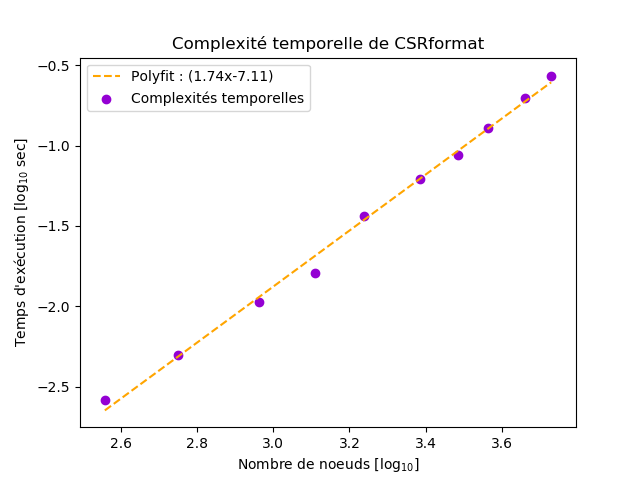
\includegraphics[width=\textwidth]{res/plots/CSR.png}
\end{minipage}
\begin{minipage}{0.5\textwidth}
Pour réaliser le passage en format creux (CSR) de la matrice, la fonction \python{CSRformat} doit localiser tous les élements non-nuls de la matrice, pour se faire elle doit parcourir toute la matrice pleine, ce qui nous donne une complexité en $\Theta(n^2)$. Ensuite cette fonction fait la somme d'éléments non-nuls par ligne et fait une somme cumulative par nombre d'éléments non-nuls par ligne pour trouver le vecteur \python{iA}. Cette complexité est menée par le parcours de la matrice, comme nous pouvons le remarquer ci à gauche, nous obtenons une pente d'environ 2 pour la régression linéaire en logarithme. L'algorithme est décrit ci-dessous.
\end{minipage}
\lstinputlisting[language=Python, firstline=1, lastline=11]{res/py/LUcsr.py}

\section{LU creuse}
\label{sec:LUcsr}

\subsection{Factorisation}
\label{sub:LUfac}

\subsubsection{Explication}
\label{subsub:LUexp}

Pour faire cette décomposition, il est tout d'abord nécessaire d'avoir une matrice creuse sous format CSR. Ensuite, il nous faut connaître la largeur de la bande pour connaître la future taille maximale de la décompostion, en effet, lors de la décomposition LU, seul les éléments contenu dans la bande (même nuls) peuvent être modifiés dû au \textit{fill-in} du \textit{outer product}. Une fois cette taille connue, nous pouvons allouer des vecteurs pouvant contenir tous les élements de la bande. Pour connaître l'élément \python{(i,j)} correspondant au bon élément dans \python{sLU}, une fonction \python{get(i,j)} a été créée, elle peut prendre en argument soit deux entiers, soit deux vecteurs d'entiers, ce qui aura pour but de se passer de boucle lors du outer product et ainsi rendre la décomposition plus rapide. Ensuite on peut donc faire un mapping entre les éléments initiaux et les vecteurs représentant la matrice \python{LU} (copier/coller).

\begin{minipage}{0.5\textwidth}
\newcommand{\scale}{1}
\[
    \left(\begin{gathered}
    \tikzpicture[every node/.style={anchor=south west}]
      \node[minimum width=1cm,minimum height=1cm] at (\fpeval{0*\scale},\fpeval{5*\scale}) { $A_{00}$ };
      \node[minimum width=1cm,minimum height=1cm] at (\fpeval{1.5*\scale},\fpeval{5*\scale}) { $V_0$ };
      \node[minimum width=1cm,minimum height=1cm] at (\fpeval{0*\scale},\fpeval{3.5*\scale}) { $V_1$ };
      \node[minimum width=1cm,minimum height=1cm] at (\fpeval{1.5*\scale},\fpeval{3.5*\scale}) { $Outer$ };
      \node[minimum width=0.1cm,minimum height=0.1cm] at (\fpeval{0.5*\scale},\fpeval{0.5*\scale}) { \Huge{0} };
      \node[minimum width=0.1cm,minimum height=0.1cm] at (\fpeval{5*\scale},\fpeval{5*\scale}) { \Huge{0} };
      \draw[dashed] (\fpeval{0*\scale},\fpeval{3*\scale}) -- (\fpeval{3*\scale},\fpeval{0*\scale});
      \draw[dashed] (\fpeval{3*\scale},\fpeval{6*\scale}) -- (\fpeval{6*\scale},\fpeval{3*\scale});
      \draw (0,\fpeval{6*\scale}) rectangle (\fpeval{1*\scale},\fpeval{5*\scale});
      \draw (0,\fpeval{3*\scale}) rectangle (\fpeval{1*\scale},\fpeval{5*\scale});
      \draw (\fpeval{1*\scale},\fpeval{6*\scale}) rectangle (\fpeval{3*\scale},\fpeval{5*\scale});
      \draw (\fpeval{1*\scale},\fpeval{5*\scale}) rectangle (\fpeval{3*\scale},\fpeval{3*\scale});
    \endtikzpicture
    \end{gathered}\right)
\]
\end{minipage}
\begin{minipage}{0.5\textwidth}
        Et enfin, on peut réaliser la décomposition composée d'une itération sur les n éléments diagonaux $A_{ii}$ (pivots) et qui à chaque itération vient diviser la colonne sous le pivot ($V_1$) par ce même pivot et ensuite vient soustraire toute la matrice carrée contenue à droite et sous l'élément diagonale par le \textit{outer product} de la colonne contenue sous le pivot avec la ligne à droite du pivot ($V_0$). La force avec les matrices bande creuses est que le \textit{outer product} va se faire seulement jusqu'à l'index maximal entre la borne droite et gauche de la bande et ainsi agir que sur une petite sous-matrice contenue dans les bornes de la bande. L'algorithme de la décomposition se trouvant ci dessous :
\end{minipage}

\lstinputlisting[language=Python]{res/py/LUfact.py}

\subsubsection{Complexité temporelle}
Sous format CSR, la largeur de la bande a de l'importance pour la complexité, elle dépend de la borne à gauche (notée \textit{g}) par rapport à la diagonale et de la borne à droite (notée \textit{d}) toujours par rapport a cette même diagonale avec $l=max(g,d)+1$.
Cette complexité temporelle dépend de différentes étapes: tout d'abord le calcul de la largeur de la bande qui est simplement le parcours par ligne : $\Theta(n)$, ensuite l'allocation des vecteurs \python{sLU}, \python{iLU} et \python{jLU} de complexité maximale $O(n(2l+1)+1)\subseteq O(nl)$ et enfin la décomposition de complexité maximale (décrite au point 2.1.1) $$O\left( \sum_{i=1}^n\left( \sum_{j=i+1}^{min(i+g,n)} + \left( \sum_{k=i+1}^{min(i+g,n)}\right)\left( \sum_{m=i+1}^{min(i+d,n)}\right)\right)\right)\subseteq O(n(g+gd)) \subseteq O(nl^2)$$
%  ADD PLOT COMPLEXITY EN LOGARITHME (SLOPE)

\subsection{Résolution}
\label{sub:LUres}
\subsubsection{Explication}
Pour cette résolution, nous devons d'abord factoriser en \python{LU} comme décrit ci-dessus et ensuite faire une substitution avant pour $Lu=b$ et enfin une substitution arrière pour $Ux=y$.
\subsubsection{Complexité temporelle}
Comme sus-mentionné, nous avons deux substitutions, ainsi la complexité de ces deux substitutions à la suite donne:
$$O(\text{Sub. avant} + \text{Sub. arrière}) = O\left( \sum_{i=1}^{n} \sum_{j=max(0,i-g)}^{i-1} +  \sum_{i=1}^{n} \sum_{j=i+1}^{min(i+d,n)}\right) \subseteq O(ng + nd) \subseteq O(nl)$$
Étant donné qu'il est nécessaire de d'abord factoriser, la complexité totale de la résolution nous donne:
$$O(nl^2+nl) \subseteq O(nl^2)$$
\subsubsection{Précision}
\begin{minipage}{0.40\textwidth}
    La fonction sous format creux et avec les noeuds renumérotés a une précision proche de celle donnée par \textit{Numpy linalg solve}, cependant lorsqu'il n'y a pas de renumérotation, plus de calculs sont faits et les erreurs d'arrondis s'accumulent, amenant à une précision moindre.
\end{minipage}
\begin{minipage}{0.60\textwidth}
    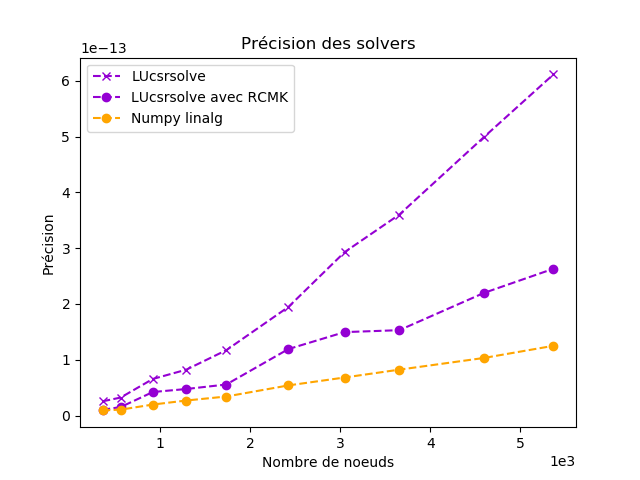
\includegraphics[width=\textwidth]{res/plots/accuracy.png}
\end{minipage}
\section{RCMK \lbrack Reverse Cuthill-McKee\rbrack}

Étant donné que la complexité temporelle de \python{LUcsrsolve} dépend de la largeur de la bande, il serait intéressant de réduire la largeur de la bande. L'algorithme \python{RCMK} vient réaranger les noeuds du problème pour densifier la bande la matrice et ainsi avoir une largeur de bande moindre.

\label{sec:RCMK}
\subsubsection{Influence sur la densité de la factorisation}
\label{sub:band}
\begin{minipage}{0.5\textwidth}
    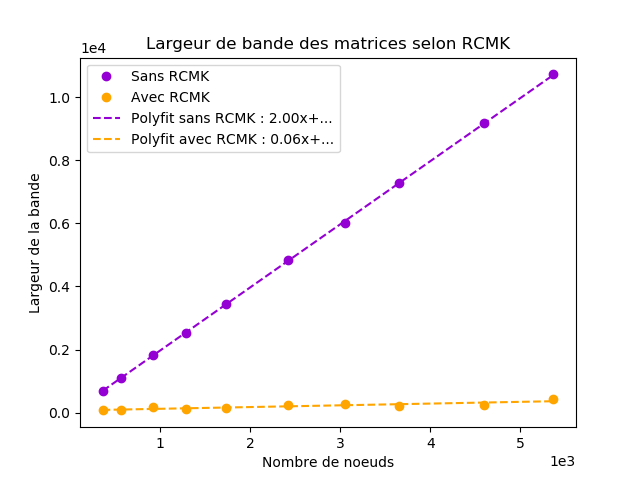
\includegraphics[width=\textwidth]{res/plots/bandRCMK.png}
\end{minipage}
\begin{minipage}{0.5\textwidth}
    Comme nous pouvons le voir ci à gauche, sans renumérotation, la largeur de la bande augmente linéairement avec le nombre de noeuds du modèle et avec une pente de 2, ce qui veut dire que la borne à gauche (resp. à droite) sus-mentionnée de la bande augmente au même taux que le nombre de noeuds augmente. Contrairement à la largeur de la bande lorsqu'il y a une renumérotation, la bande augmente avec un taux d'environ 6\% par rapport au nombre de noeuds.
\end{minipage}
\begin{minipage}{0.5\textwidth}
    \centering
    \begin{tabular}{cc}
      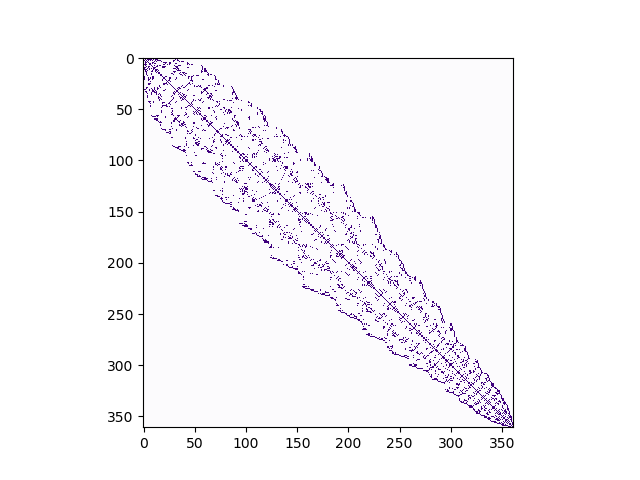
\includegraphics[width=.4\linewidth]{res/matrix/RCMK/Statique361.png} &
      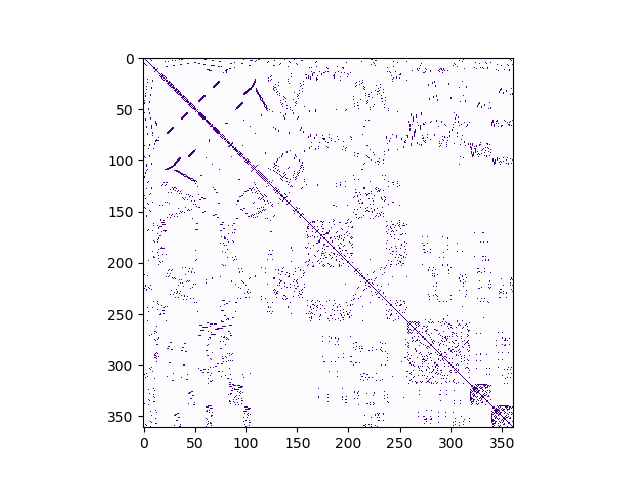
\includegraphics[width=.4\linewidth]{res/matrix/Standard/Statique361.png} \\
      (a) Avec renumérotation & (b) Sans renumérotation \\
    \end{tabular}
    La densité de la matrice A est moindre que les matrices LU avec ou sans RCMK, ce qui est normal dû au \textit{fill-in}. Ensuite, on peut remarquer que la décomposition LU sans RCMK est plus dense, dû au phénomène de \textit{fill-in} qui est plus présent dû à la largeur de bande plus grande. Enfin, on voit que cette densité diminue avec la taille du système ce qui est une priorité du modèle d'éléments finis.
\end{minipage}
\begin{minipage}{0.5\textwidth}
    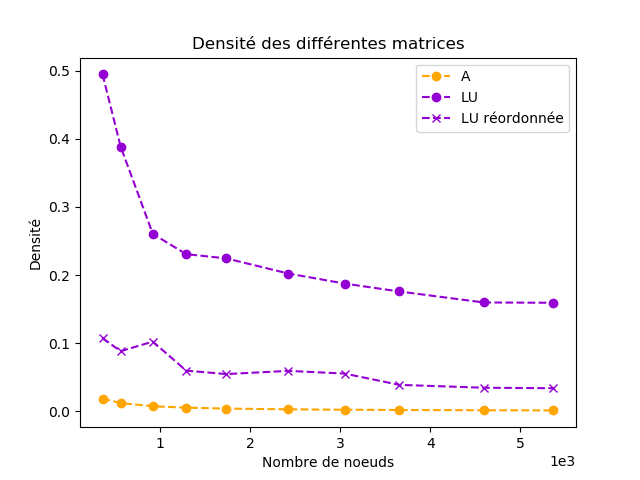
\includegraphics[width=\textwidth]{res/plots/DensityRCMK.png}
\end{minipage}

\subsubsection{Influence sur la complexité temporelle de la résolution}
\begin{minipage}{0.5\textwidth}
    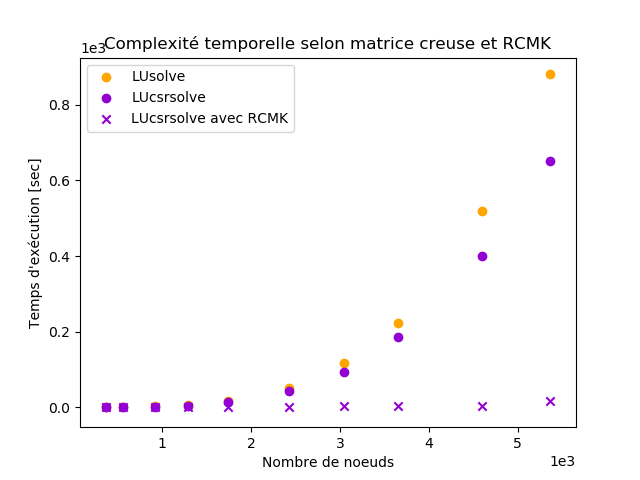
\includegraphics[width=\textwidth]{res/plots/complexity.png}
\end{minipage}
\begin{minipage}{0.5\textwidth}
    On peut donc bien remarquer que dans le cas de notre modèle d'élements finis qui est creux, la fonction de résolution par \textit{factorisation LU} sous format creux et plus performant en terme de temps de calculs. Étant donné que la bande couvre quasiment toute la largeur de la matrice lorsqu'il n'y a pas de renumérotation, elle a donc une complexité temporelle proche de la factorisation avec matrice pleine car les calculs sont quasiement identiques. Cependant lors de l'utilisation de la renumérotation, la complexité est très faible car comme indiqué au point 3.0.1 et 2.2.2, la largeur de la bande n'augmente que de 6\% par rapport aux noeuds et la complexité dépend de la largeur de bande.
\end{minipage}
\begin{minipage}{0.5\textwidth}
    De manière qualitative, on peut voir que la complexité du solver \python{LU} en format creux est d'environ $O(n^{1.6})$. Cette complexité n'est pas objective dû à toutes les fonctions numpy vectorisées.
\end{minipage}
\begin{minipage}{0.5\textwidth}
    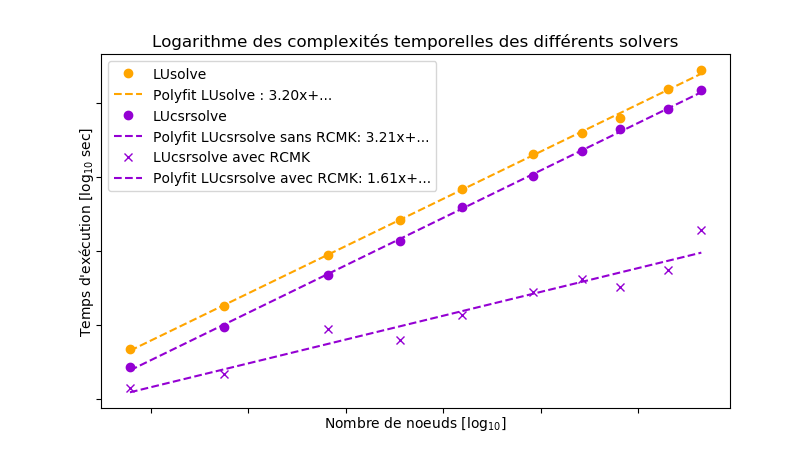
\includegraphics[width=\textwidth]{res/plots/complexitylog.png}
\end{minipage}
\section{Nécessité du pivotage}
\label{sec:pivotage}
\begin{minipage}{0.5\textwidth}
    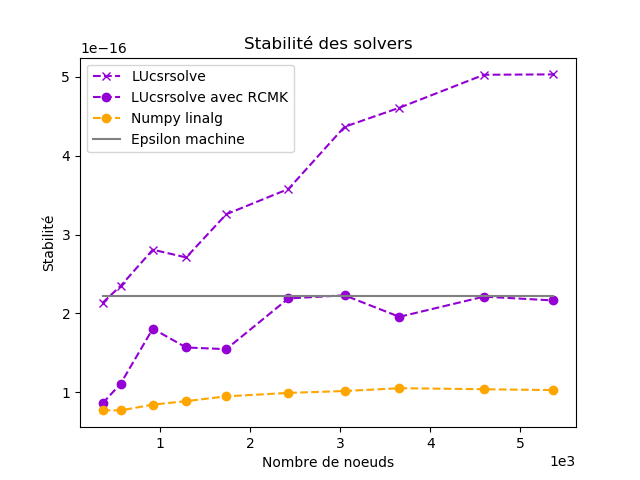
\includegraphics[width=\textwidth]{res/plots/backward.png}
\end{minipage}
\begin{minipage}{0.5\textwidth}
    Lors de l'algorithme sans renumérotation RCMK, la stabilité est semblable à l'algorithme LU dense sans pivotage, ainsi, la stabilité n'est pas optimale dû aux possibles divisions par 0 de l'élimination de Gauss. Cependant, lors de l'utilisation de la renumérotation RCMK, la bande de la matrice est bien plus dense, les éléments sont réarangés autour de la diagonale, ainsi, les divisions par 0 ne sont pas possibles et les phénomènes de \textit{fill-in} se font moins que dans la version avec les éléments disparates. La \textit{backward stability} est donc bien meilleure comme peut le montrer le graphe ci à gauche, elle est de l'ordre de O($\epsilon_{\text{machine}}$).
\end{minipage}
\end{document}
